\documentclass{article}
\usepackage[utf8]{inputenc}
\usepackage{amsmath}
\usepackage{amsfonts}
\usepackage{stmaryrd} % more math symbols
\usepackage{amsthm} % for theoreme style


%%%% for images
\usepackage{graphicx}
\graphicspath{ {./rapports} }

%%%% to set boxes like a theorem
\theoremstyle{definition}
\newtheorem{definition}{Definition}[section]

\theoremstyle{property}
\newtheorem{property}{Property}[section]

\theoremstyle{remark}
\newtheorem*{remark}{Remark}
%%%% to insert a line of code in the text with \texttt{ code }
\newcommand{\code}[1]{\texttt{#1}}


\title{Idées polynomes}
\date{January 2022}

\begin{document}
	\section{Find F}
	Set $(d,n)\in \mathbb{N}^*$ and $(x_i)_{i\in \llbracket0;n-1\rrbracket }\in \mathbb{R}^{d}$ distinct one another. We seek a polynomial $F\in\mathbb{K}[X]$ such that $\mathbb{K} \in \{\mathbb{R},\mathbb{C}\}$ and
	$$\forall i\in \llbracket1;n\rrbracket,~F(x_i)=0 \text{ and } \exists x_n:~F(x_n)\neq0$$
	
	\subsection{Case 1D}
	In the case $d=1$, Vandermonde polynomials are a good start. The only thing to add to the construction is a point where the polynomial $F$ is not null. Assuming the orthobarycentre of the family $(x_i)_{i\in \llbracket0;n-1\rrbracket }$ is not already inside, let's take the orthobarycentre of these points defined as $x_n:=\frac{1}{n}\sum_{i=0}^{n-1} x_i$.\\
	The system induced is this one :
	\begin{equation*}
		\begin{pmatrix}
			1 & x_0 & \dots & x_{0}^{n} \\
			\vdots & \vdots & \ddots & \vdots\\
			1 & x_{n-1} & \dots & x_{n-1}^{n} \\
			1 & x_n & \dots & x_n^{n-1} 
		\end{pmatrix}
		\begin{pmatrix}
			a_0\\
			\vdots\\
			a_{n-1}\\
			a_{n}
		\end{pmatrix}
		=
		\begin{pmatrix}
			0\\
			\vdots\\
			0\\
			1
		\end{pmatrix}
	\end{equation*}
	that one can solve thanks to the inversion of the Vandermonde matrix, which is non-singular since all the points are distinct one another thanks to the assumption.
	
	
	\subsection{Case 2D}
	The work done here for $d=2$ is meant to be easily generalizable to even greater values of $d$.
	Set $\forall i \in \llbracket0;n-1\rrbracket, x_i \text{ has as coordinates }(x_{i,0},x_{i,1})$.
	
	\subsubsection{Matrix method}
	\subsubsection*{Start of an idea (inspired from Vandermonde matrix in 1D)}
	Globally, $F$ can be defined in $\mathbb{R}_{n+1}[X]$ considering its roots $(x_i)_{i\in \llbracket0;n-1\rrbracket }$ and the point $x_n$ where it is not null. Therefore, set $x_n$ the orthobarycentre with the same assumption as previously 	and $(\alpha_{ij})_{\{(i,j)\in\mathbb{N}:i+j\leq n\}}\in\mathbb{R}^{2n}$ such that
	\begin{equation*}
		\forall (x,y) \in \mathbb{R}^2,~F(x) = \sum_{\{(i,j)\in\mathbb{N}:i+j\leq n\}} \alpha_{ij}x^iy^j
	\end{equation*}
	\begin{equation*}
		\begin{pmatrix}
			1 & x_{0,0} & x_{0,1} & x_{0,0}x_{0,1} & \dots & x_{0,1}^{n} \\
			\vdots & \vdots&\vdots & \vdots& \ddots & \vdots \\
			1 & x_{n-1,0} & x_{n-1,1} & x_{n-1,0}x_{n-1,1} & \dots &x_{n-1,1}^{n} \\
			1 & x_{n,0} & x_{n,1} & x_{n,0}x_{n,1} & \dots & x_{n,1}^{n} \\
		\end{pmatrix}
		\begin{pmatrix}
			\alpha_{00}\\
			\vdots\\
			\alpha_{0(n-1)}\\
			\alpha_{0n}
		\end{pmatrix}
		=
		\begin{pmatrix}
			0\\
			\vdots\\
			0\\
			1
		\end{pmatrix}
	\end{equation*}
	Actually, Vandermonde does not give any proof of the non-singularity of the left matrix and one could thought about putting more combinations of the coordinates of each point to extract a non-singular matrix after.
	Yet, finding this extracted matrix remains computationally heavy in addition to being uncertain.\\
	
	\subsubsection*{In hindsight}
	The realm this idea steps into is the realm of principal component analysis. It remains interesting considering the fast differentiation of the polynomial one could get after. Nevertheless, it could force us to already use machine learning which will require some time to compute accurately and will always remain an approximation of the true solution we seek.

	
	\subsubsection{Direct approach}
	In this kind of situation, constructing the polynomial $$F:(x,y)\mapsto\prod_{m=0}^{n-1}(x-x_i)(y-y_i)$$ quickly comes to mind. Nevertheless, $F$ would be to often null on the domain and could induce great errors after. So, the idea is to replace the given factor by one null only at a given point as shown here:
	\begin{definition}\label{F_real}
		$$\forall (x,y)\in\mathbb{R}^2,~F_r(x,y) = \prod_{k=0}^{n-1}((x-x_k)^2 + (y-y_k)^2)$$
	\end{definition}
	
	\begin{definition}\label{F_comp}
		$$\forall (x,y)\in\mathbb{R}^2,~F_c(x,y) = \prod_{k=0}^{n-1}((x-x_k) + i(y-y_k))$$
	\end{definition}
	
	\begin{remark}[comparison]\
		\begin{itemize}
			\item $\forall (x,y)\in\mathbb{R}^2,~F_r(x,y)=\vert F_c(x,y) \vert^2$
			\item the coefficients of $F_c$ are faster to compute but harder to evaluate than the ones of $F_r$
		\end{itemize}
		
	\end{remark}
	
	\newpage
	\section{Hyperparameters}
	Here is the scheme of model tuning followed:
	\begin{figure}[h]
		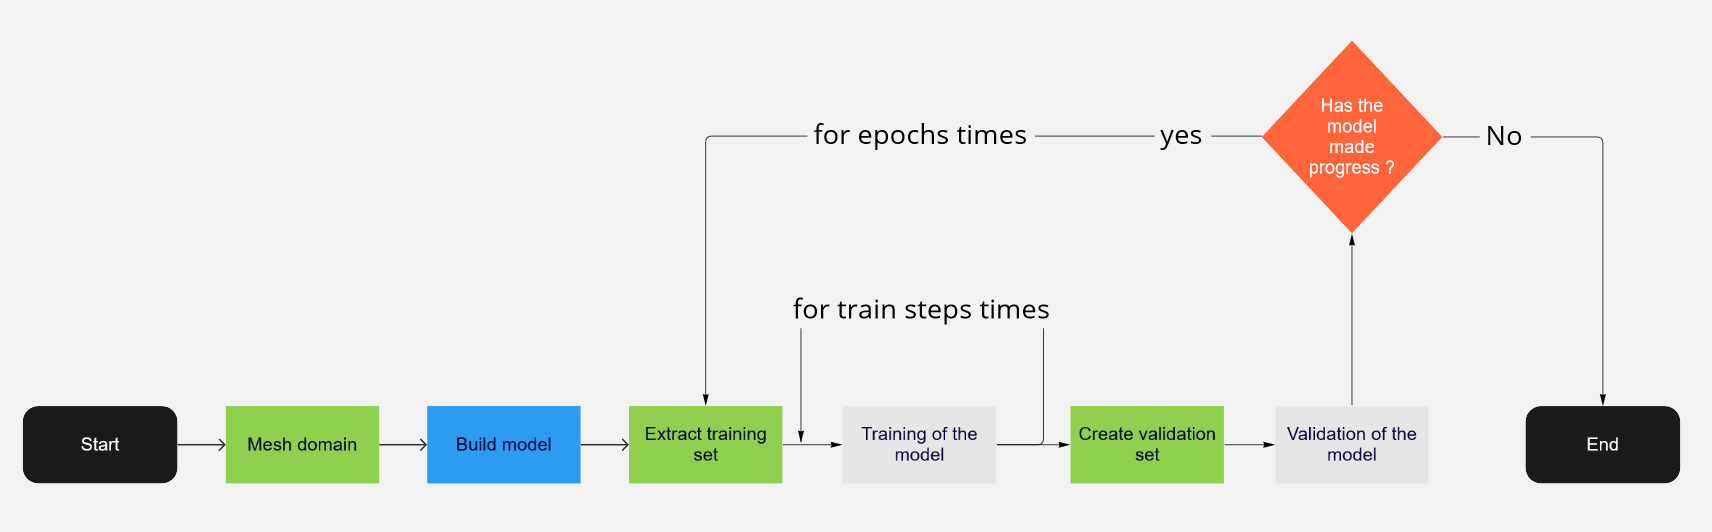
\includegraphics[width=13cm, height=4cm]{tuning_model.png}
		\centering
		\caption{scheme of a model tuning}
	\end{figure}
	\begin{remark}
		The red box involves using an early stopping callback to stop the epoch loop when the model begins to overfit. A \texttt{patience} integer set how far the system will go back in history. If during \texttt{patience} epochs the has not made progress the epoch loop is stopped.
	\end{remark}
	
	The hypertuning comes when one wants to construct a model and a training that will end to a low validation error. Let's list all the hyperparameters involved in this scheme applied for the Poisson equation on a square domain:
	\begin{itemize}
		\item \texttt{grid\_length}: integer setting the number of points in the domain to \texttt{grid\_length}x\texttt{grid\_length}
		\item \texttt{l\_units}: list of integers depicting the number of hidden layers and the number of neurons per layer of the sequential machine learning model
		\item \texttt{l\_activations}: list depicting the activation functions of each layer of the model
		\item \texttt{noise}: integer in $\{0,1\}$ conditioning the use of a Gaussian layer of mean $0$ after the input layer
		\item \texttt{stddev}: the standard deviation of the Gaussian layer when it is used
		\item \texttt{optimizer}: string depicting the optimizer used
		\item \texttt{learning\_rate}: float setting the learning rate of the previous optimizer
		\item \texttt{epochs\_max}: integer setting the number of maximum epoch loops
		\item \texttt{n\_trains}: integer setting the number of train loops
		\item \texttt{batch\_size}: integer setting the number of points extracted from the mesh to construct the training set at each epoch loop
		\item \texttt{patience}: integer setting how many epoch loops the system can go on without progressing, after that the trial is ended
	\end{itemize}
	
	Some work must still be done to assure a low validation error with minimal cost of time and hardware. A few bugs impeding a proper convergence seems to still persist in some of our implementations.
	
	
	
\end{document}
